\documentclass{scrartcl}
\usepackage{graphicx}
\usepackage{rotating}
\usepackage{hyperref}
\usepackage{textcomp}
\usepackage[left=2.3cm,right=2.3cm,top=2.5cm,bottom=2cm,includeheadfoot]{geometry}

\title{Pollux Astro Powerbox Operating Manual}
\author{Philipp Weber \\
  \footnotesize{\href{mailto:philipp@whyisitso.dep}{philipp@whyisitso.de}}
}

\begin{document}

\maketitle
\newpage

\tableofcontents
\newpage

\section{Disclaimer}
Although I am doing my best to create a good and helpful project, it is
distributed in the hope that it will be useful, but WITHOUT ANY WARRANTY;
without even the implied warranty of MERCHANTABILITY or FITNESS FOR A PARTICULAR
PURPOSE. See the GNU General Public License for more details. Please understand
that you are using the device AT YOUR OWN RISK and I can not be responsible for
any damage created by using it.


\section{Features}
The powerbox acts as a power distribution and dewheating system which can be
controlled using either \texttt{INDI} or \texttt{ASCOM} and also supplies
environmental information to the imaging software with the following features:
\begin{itemize}
  \item Input voltage measurement
  \item Environmental information:
    \begin{itemize}
      \item Temperature
      \item Pressure
      \item Relative humidity
      \item Dewpoint
    \end{itemize}
  \item Power distribution:
    \begin{itemize}
      \item Reverse polarity protection
      \item Four combined switchable 12\,V outputs
      \item One always on 12\,V output
      \item One adjustable output from 5\,V to 12\,V
    \end{itemize}
  \item Two independent dewheaters:
    \begin{itemize}
      \item Reference temperature from probes on the heater strips
      \item No unnecessary power consumption
      \item Different working modes based on environmental parameters
      \item Built in PID controller for each heater
      \item PWM controlled output power
      \item Adjustable constant heater power possible
    \end{itemize}
  \item All outputs protected by self-resetting fuses
  \item All settings stored directly on the device
  \item Possible operation without PC control
  \item Unique serial ID from the CH340B USB to serial converter
\end{itemize}

\section{Connectors and Electrical Parameters}
\subsection{Device Description}
The following image and table give a list of connectors of the powerbox.
\begin{figure}[ht!]
  \centering
  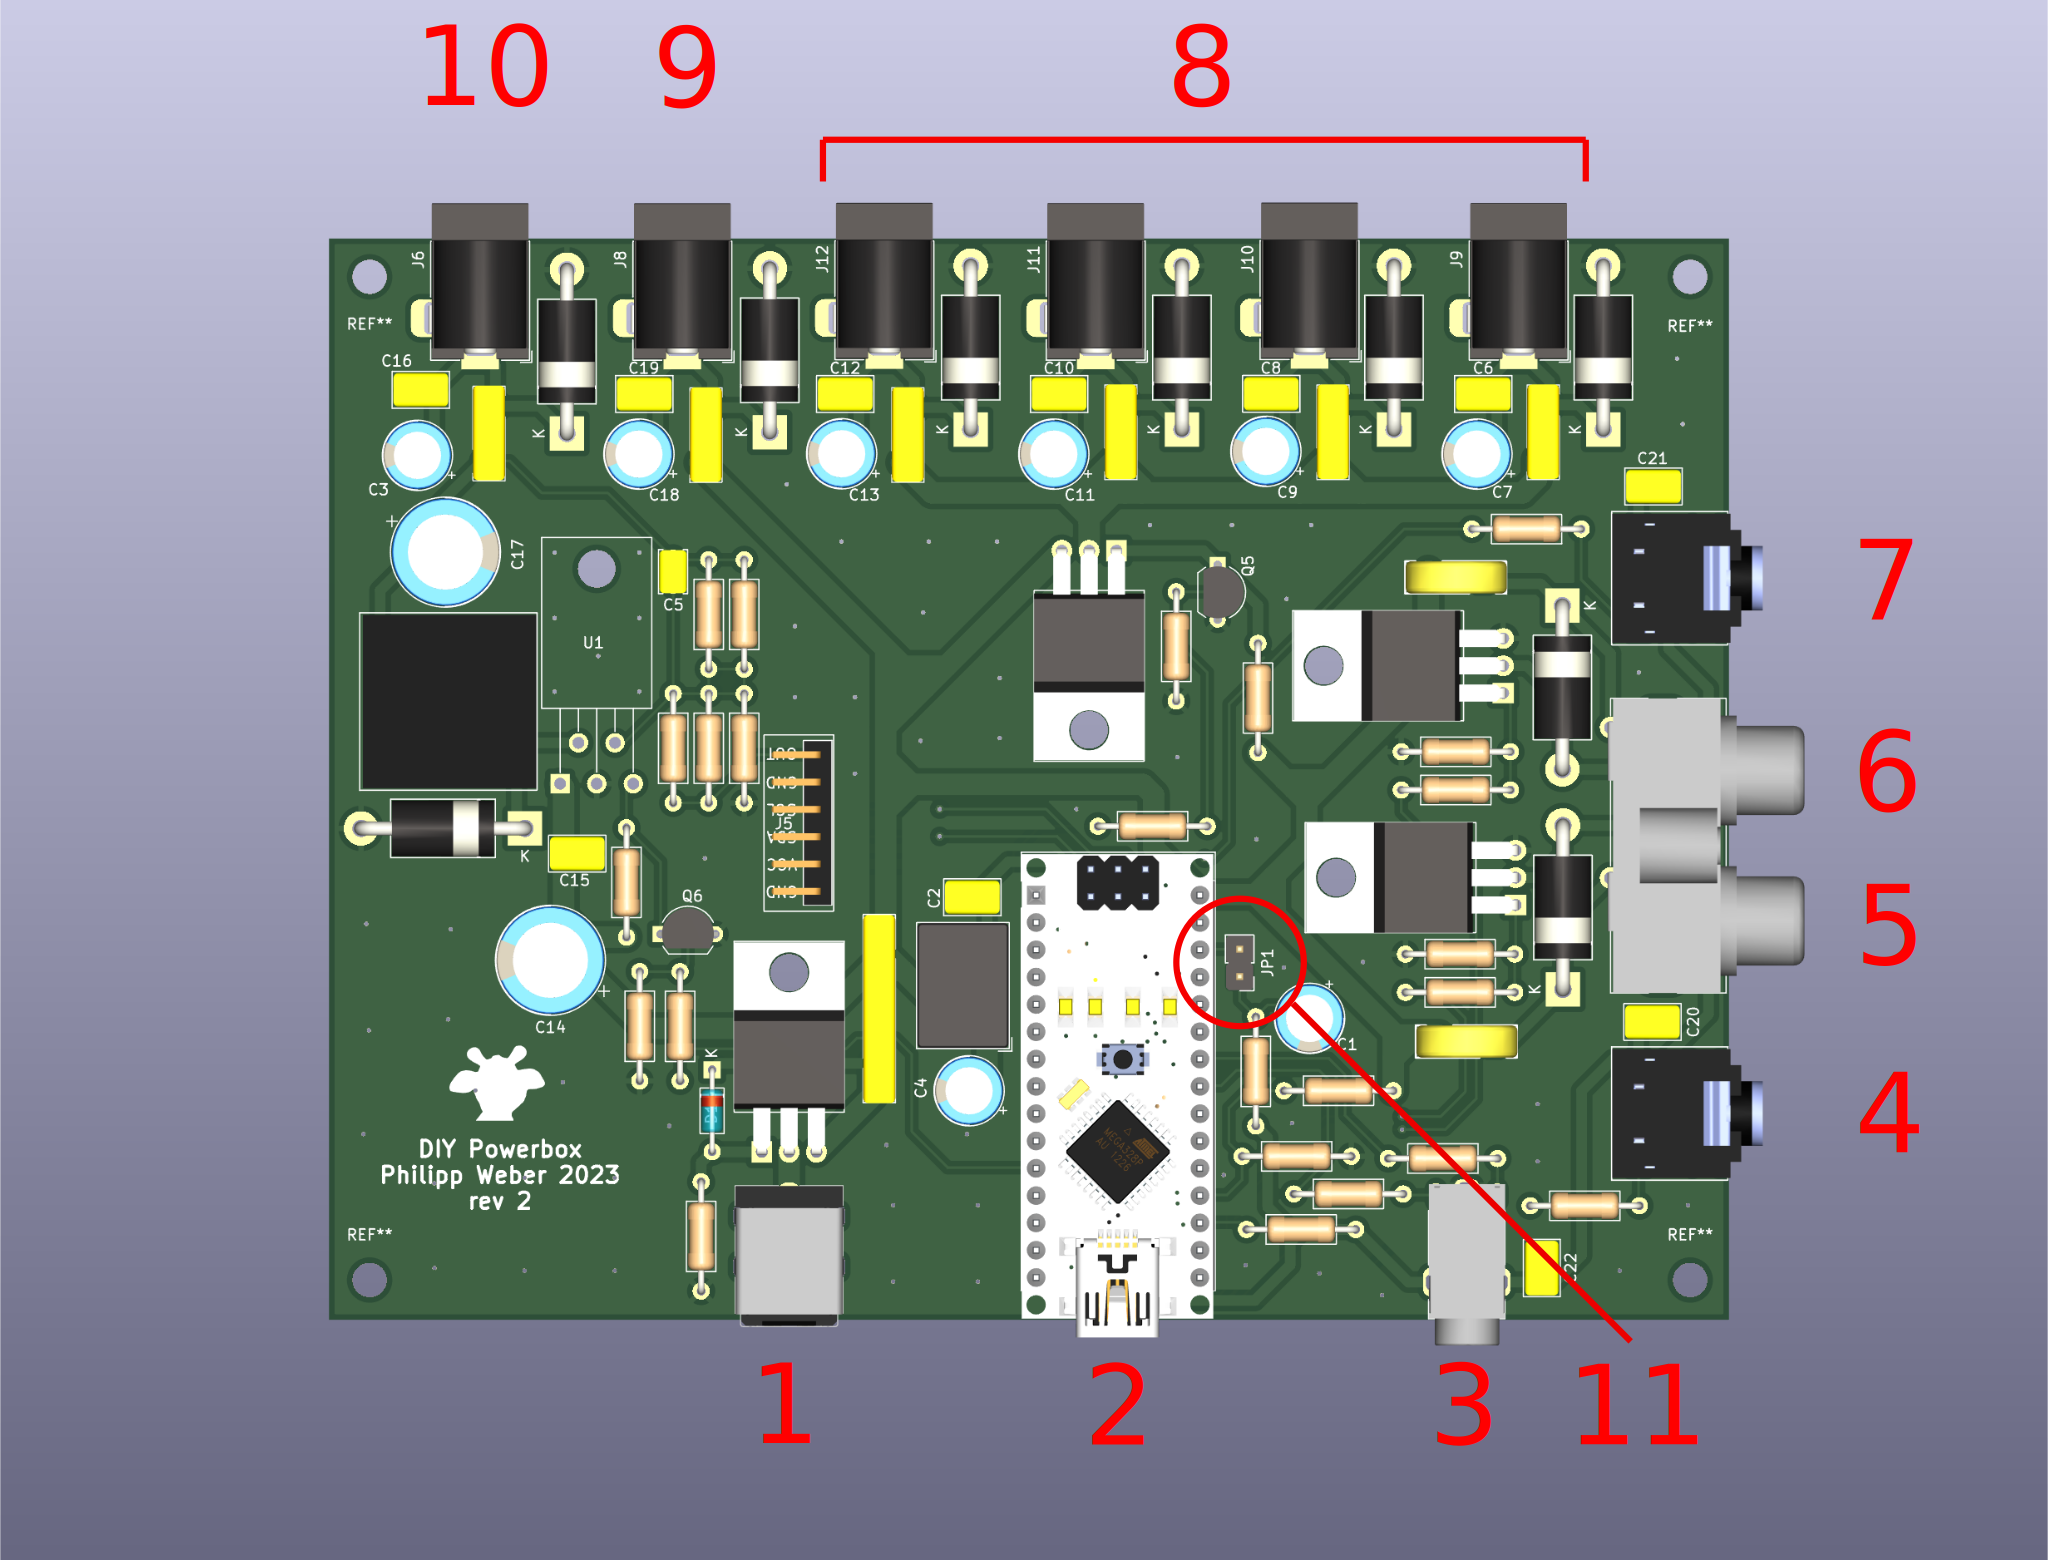
\includegraphics[width=0.7\textwidth]{powerbox.pdf}
  \caption{Main connectors of the powerbox}
  \label{fig:powerbox}
\end{figure}
\begin{table}[ht!]
  \centering
  \caption{Connectors and their properties as marked in Fig.~\ref{fig:powerbox}}
  \begin{tabular}{lcccc}
    \textnumero & Connector & Voltage [V] & Fuse [A] & Purpose \\
    \hline \\
    1  & 2.1\,mm/5.5\,mm barrel jack   & 12 \ldots 16      & 10     & Input power ($V_{\mathrm{in}}$) \\
    2  & USB-C                         & 5                 & n/a    & Computer control \\
    3  & 4x3.5\,mm headphone jack      & 5                 & n/a    & External environment sensor \\
    4  & 3x3.5\,mm headphone jack      & 5                 & n/a    & Dewheater 1 temperature probe \\
    5  & Cinch                         & $V_{\mathrm{in}}$ & 2      & Dewheater 1 output \\
    6  & Cinch                         & $V_{\mathrm{in}}$ & 2      & Dewheater 2 output \\
    7  & 3x3.5\,mm headphone jack      & 5                 & n/a    & Dewheater 2 temperature probe \\
    8  & 4x2.1\,mm/5.5\,mm barrel jack & $V_{\mathrm{in}}$ & 3 each & Switchable output rail \\
    9  & 2.1\,mm/5.5\,mm barrel jack   & $V_{\mathrm{in}}$ & 3      & Always on  \\
    10 & 2.1\,mm/5.5\,mm barrel jack   & 5 \ldots 12       & 3      & Adjustable output \\
    11 & Jumper                        & 5                 & n/a    & Remove to program \\
    \hline
  \end{tabular}
\end{table}

\subsubsection{Input Voltage}
As long as the input voltage stays above 6.5\,V the device is expected to
operate normally, but it is recommended for the input voltage to be at least
12\,V. The fuses are rated for a voltage of 16\,V, but all other parts up to
25\,V.
\begin{quote}
  \textbf{
16\,V should be considered the absolute maximum value the device can
operate at, but it is still recommended to keep the input voltage in the range
from 12\,V to 16\,V.
}
\end{quote}
Increasing the input voltage above 16\,V can damage the device.

The input connection is protected by a self-resetting fuse with a specified
hold-current of 10\,A, as well as a reverse polarity protection.

\subsubsection{USB Connection}
The socket for the USB connection to the computer is a USB 2.0 type C socket
provided by the Arduino Nano in the powerbox. This digital connection ends with
the USB to serial (RS-232) converter chip on the Arduino. From this point the
serial connection is implemented to the microcontroller with roughly 2\,cm long
traces on the PCB. This connection is not subject to integrity checks on the
hardware level and therefore errors in the transmission over this short distance
are theoretically possible. To mitigate this problem the firmware on the
microcontroller and the driver running on the PC implement checksum algorithms
to detect those errors in the transmission. The serial connection is running at
a baud rate of 115200\,Baud.

An additional problem can be caused by multiple such microcontrollers being
connected with a serial connection to a computer if they don't have a unique
hardware ID. In such a case the computer can not distinguish between these
devices and picking the correct one becomes a game of chance. For this reason
the RS-232 to USB converter in the powerbox uses the CH340B chip, each of which
has a unique ID making it possible to repeatedly pick the same device in case
multiple such converters are connected.

\subsubsection{External Sensor}
For the dewheater to operate correctly the firmware needs to know about the
environmental conditions, most importantly the dewpoint, which is the
temperature the air has to reach with the current humidity to be saturated with
water vapor, at which point fog and dew can form. For this calculation the
current air temperature, the relative humidity, and the air pressure are
necessary. These values are provided by the BME280 sensor from Bosch, located on
the external sensor board. It is connected to the main device via a cable with 4
pin 3.5\,mm headphone jacks.
\begin{quote}
\textbf{
  It is absolutely vital that the environment sensor is located at a place where
  it is not subject to any source of heat. It must only measure the properties
  of the ambient air.
}
\end{quote}
Note that if the external sensor board is not properly connected the device
will not operate correctly.

\subsubsection{Dewheater Outputs and Probes}
The sockets of the two dewheater channels are standard Cinch connectors with the
positive connection on the center pin. Each of the channels is protected by a
separate 2\,A fuse, translating to a maximum power output of each channel of
24\,W.
\begin{quote}
  \textbf{
    Always make sure to only use dewheater elements which consume at most 24\,W of
    power.
  }
\end{quote}
The algorithms for the dewheater control implemented in the firmware rely on the
knowledge of the current temperature of each active dewheater. To this end at
most two DS18B20 temperature probes, one for each channel, can be placed on the
dewcap(s) of the telescope(s) alongside the dewheater strips. Each of these
temperature probes is connected to the main device via a 3-pin headphone jack.
Each temperature probe connector corresponds to the dewheater channel it is
located next to on the housing of the main device. For more information on the
dewheater operation see section~\ref{sec:dewheater}.

\subsubsection{4x12\,V Rail}
Each of the 4 outputs of the 12\,V rail is protected by its own self-resetting
fuse with a specified hold-current of 3\,A. All of these 4 outputs can be
switched on or off together. The output voltage of these ports is identical to
the input voltage.

\subsubsection{Always On}
As the name implies, the ``always-on'' port is always supplied with power. It is
intended for the operation of a USB-Hub, trough which the powerbox itself is
connected to the controlling computer. If it was connected to, for example, one
of the ports of the 12\,V rail, and this is switched off, the USB connection to
the powerbox might be interrupted and the rail can potentially not switched on
again. By having a constant supply of power to the USB-hub this problem can be
omitted.

The always-on port is also protected with a self-resetting fuse with a
hold-current of 3\,A. The output voltage of this port is identical to the input
voltage.

\subsubsection{Adjustable Output}
Some devices, for example DSLR cameras, do not require a supply of 12\,V but
less, and exceeding that voltage could damage such devices permanently.
Therefore the powerbox is equipped with an output port which can supply an
arbitrary voltage between 5\,V and 12\,V (technically a bit less than 12\,V).
This voltage can be adjusted steplessly through the \texttt{ASCOM} or
\texttt{INDI} drivers. Additionally, the output can be switched on or off
completely, independently of the voltage setting.

The adjustable output is also protected by a self-resetting fuse with a
hold-current of 3\,A.

\subsection{A Note on Power Plugs}
The most commonly used connector for astronomy equipment is the barrel jack. Its
receptacle consists of a central pin and a spring loaded contact. The plug has a
central hole in which the pin of the receptacle resides, and a sleeve which the
outer contact of the receptacle touches. It is almost always assumed that the
positive terminal of the power supply as well as the device is connected to the
central pin, and the negative terminal, i.e. ground, is connected to the sleeve.
The same assumption is true for all barrel jack connectors of the powerbox, as
well as the Cinch connectors for the dewheaters.

Additionally, the sizes of the central pin and that of the outer sleeve can
vary. The most common sizes are 2.1\,mm for the pin and 5.5\,mm for the sleeve.
These are the dimension of all power plugs of the powerbox. Also pins with
2.5\,mm diameter are common. The respective plugs will also fit in the
receptacles of the powerbox (given the sleeve diameter is the same), but contact
can not be guarenteed, and the plugs will not have a good fit in the receptacle
and may fall out.

Of course also the current rating of the plugs, as well as the cables, must be
considered. This is especially important for the power input connection of the
powerbox. The receptacle and the PCB are designed to handle at least 10\,A of
current at 12\,V. If this capacity is expected to be saturated also the cable
and plug supplying the current must be rated accordingly. If not the input
voltage might drop, or the cable or the plug might heat up, and in the worst
case melt or even catch on fire. So please make sure to choose the supply line
accordingly.

\subsection{Self-Resetting Fuses}
All power outputs of the powerbox, these are the 4x12\,V switchable outputs, the
always on 12\,V output, the adjustable output, and the dewheater outputs, have
their dedicated self-resetting fuses, so called ``polyfusese''. Also the input
line of the powerbox is protected with a dedicated polyfuse. These fuses
drastically increase their resistance upon an increase in temperature, which is
generated by a large amount of current through the fuse. Depending on the amount
of overcurrent it may therefore take a small number of seconds for the fuse to
actually trigger. As soon as the overcurrent condition is fixed the fuse will
reset itself within minutes or hours. If the overcurrent situation is not
resolved a small amount of current ($< 100\,\mathrm{mA}$) will keep flowing
through the fuse to keep the temperature high and the fuse in the tripped state.

\subsection{Accuracy of the Voltage Reading and Adjustable Output}
The reading of the input voltage and the value of the output voltage of the
adjustable outputs are created using networks of several resistors. To get these
values as accurately as possible resistors with a tolerance of 0.1\% were
chosen, but this is still not enough to ensure perfect values for these
voltages. It is expected that the readings can be off by as much as $\sim
0.2\,\mathrm{V}$.

\subsection{Voltage Stability}
An electronic device consuming power can change the amount of power it requires
on a very short notice. Modern regulated power supplies are design to correct
for such changes in the required current on timescales of milliseconds, but
during this short period the potential change in the supply voltage can affect
other devices connected to the same power supply. In order to protect all
devices connected to the powerbox from such a condition every output is equipped
with its own set of decoupling capacitors. Large, 100\,$\mu$F electrolyte
capacitors can compensate to some degree for changes in the required amount of
current from devices, while small, 100\,nF ceramic capacitors can filter
short-term fluctuations resembling electronic noise.

In case a capacitive load is connected to one of the outputs, for example a fan,
which can store energy, that energy can enter the powerbox in the reverse
direction if the device is turned off. This can cause a short term internal
reverse polarity condition which can be harmful to other connected devices or the
powerbox itself. To mitigate this problem each output is equipped with a so
called ``free-wheeling diode'' which is deliberately placed in the opposite
direction to the normal current flow. If a capacitive load causes a reverse
polarity condition a closed loop is generated by the diode, essentially shorting
the device and protecting the remaining circuit. Normally this condition is not
harmful to the device causing the situation as well, because it is not connected
to a power supply anymore and the current drops very quickly.

\section{Dewheater Operation}
\label{sec:dewheater}
For observations it is absolutely vital that all optical surfaces remain clear
of dew. To this end the powerbox implements several different mechanisms to
control two heating elements like dew heater strips via pulse-width modulation.
To make use of these heating elements most efficiently the controlling firmware
needs to have knowledge of the temperature the heated element has reached. This
temperature is fed back into the PID controller of the powerbox in order to
reach a sufficiently high temperature while at the same time not wasting any
useless energy.

Please note that these temperature probes are not necessarily required to
operate the dewheaters or the device as a whole. Especially when only one of the
two dewheater channels is being used the probe for the other channel can simply
be omitted. However, if a dewheater mode (see below) is being used, that
requires the knowledge of the probe's temperature, and the probe is not
available, the corresponding channel will switch the output to 100\% for safety
reasons.

\subsection{Placing the Temperature Probes}
The two probes are water proof and sealed DS18B20 temperature probes with small
stainless steel tubes at each end. In case a dewheater strip is being used the
corresponding temperature probe can simply be tucked between the strip and the
dew shield of the telescope. The probe will then read a temperature
somewhere between the temperature of the dew shield and that of the heater strip
itself. The remaining nuances regarding temperature differences must be set with
the options for the operating modes listed in the following.

\subsection{Setting Temperature Offsets}
The DS18B20 probes of the dewheater channels, as well as the BME280 sensor for
the environment measurements, show some deviations in the manufacturing process
and therefore report slightly different temperatures, usually deviating by less
than $1^{\circ}$C. To correct for this slight deviation an offset for each probe
can be stored in the device via the \texttt{ASCOM} or \texttt{INDI}
interface. To determine this offset simply connect all sensors to the device \emph{but
not to any source of heat, also not the dewheater outputs}. Then wait ca.
5\,minutes and use the temperature offset for two of the sensors to adjust these
values such that they agree with the third sensor.

\subsection{Dewheater Modes}
Several algorithms are implemented to control the amount of power directed
towards the outputs of the dewheater channels, some considering the values of
the temperature probes, and some independently of that. Those modes are outlined
in the following.

The parameters for each mode are stored independently from each other in the
device when they are changed, even when this particular mode is not being used
at the time.

\subsubsection{Fixed Mode}
\label{sec:dewheater_fixed}
In this simple mode a dewheater channel is set to a fixed ratio of its total
output power, expressed in percent. The total power is determined by the wattage
of the heating element. This mode does not require a temperature probe.

\subsubsection{Dewpoint Mode}
In this mode, which requires a temperature probe, the powerbox will adjust the
power to the heating element of a given dewheater channel such that the measured
temperature of that channel's probe is above the calculated dewpoint by an
adjustable margin expressed in $^{\circ}$C. The motivation for this mode is that
as long as the temperature of the heated element is above the dewpoint it can
not form dew.

For example, if the dewpoint is $5^{\circ}$C and the setting is $3^{\circ}$C the
powerbox will keep the temperature of the heated element at $8^{\circ}$C.

\subsubsection{Ambient Mode}
In this mode, which requires a temperature probe, the powerbox will adjust the
power of the heating element of a given dewheater channel such that the measured
temperature of that channel's probe does not drop below the ambient temperature
minus an adjustable margin expressed in $^{\circ}$C. The motivation for this
mode is that the ambient temperature is always higher than the dewpoint and
therefore when keeping the temperature of the heated element close to the
ambient temperature it can not form dew.

For example, if the ambient temperature is $5^{\circ}$C and the setting is
$3^{\circ}$C the powerbox will keep the temperature of the heated element at
$2^{\circ}$C.

\subsubsection{Midpoint Mode}
In this mode, which requires a temperature probe, the powerbox will adjust the
power of the heating element of a given dewheater channel such that the measured
temperature of that channel's probe is above the point midway between the
ambient temperature and the dewpoint plus an adjustable margin expressed in
$^{\circ}$C. The motivation for this mode is a compromise between the dewpoint
and ambient mode.

For example, if the dewpoint is $9^{\circ}$C, the ambient temperature
$3^{\circ}$C, and the setting $+2^{\circ}$C, the powerbox will keep the
temperature of the heated element at $8^{\circ}$C. Please note that this setting
can also be negative.

\subsubsection{Slave Mode}
In this mode the dewheater will constantly adjust its output power to follow the
output power of the other dewheater. This mode of operation does not require a
temperature probe, but only one of the dewheater channels can use this mode at a
given time.

The motivation for this mode is a setup where one channel can rely on the
measurement of the heated element, for example a dew cap, while the other
channel can not, for example when using a heater for the secondary mirror of a
Newtonian.

\subsection{Switching a Dewheater Off}
A dewheater can be switched off by using the fixed output mode (see
section~\ref{sec:dewheater_fixed}) with a setting of 0\% output power.

\section{Headless Operation}
Whenever a setting is changed via the \texttt{ASCOM} or \texttt{INDI} driver the
device automatically stores all its settings in the onboard storage. As soon as
the device is switched off and then switched on again it tries to restore these
last saved settings and continues its operation in the same way. This includes
the settings of the power outputs and the dewheater modes.

The first time the device is switched on, or when the stored settings become
corrupted, the device automatically reverts to a set of safe settings. Those
are:
\begin{itemize}
  \item 12\,V rail: Off
  \item Adjustable output
    \begin{itemize}
      \item State: Off
      \item Voltage: 5\,V
    \end{itemize}
  \item Dewheater 1
    \begin{itemize}
      \item Mode: Dewpoint
      \item Fixed value: 0\%
      \item Dewpoint offset: $2^{\circ}$C
      \item Ambient offset: $5^{\circ}$C
      \item Midpoint offset: $5^{\circ}$C
    \end{itemize}
  \item Dewheater 2
    \begin{itemize}
      \item Mode: Dewpoint
      \item Fixed value: 0\%
      \item Dewpoint offset: $2^{\circ}$C
      \item Ambient offset: $5^{\circ}$C
      \item Midpoint offset: $5^{\circ}$C
    \end{itemize}
\end{itemize}
Also all temperature probe offsets are reset to $0^{\circ}$C.

\section{Firmware Updates}
In case a new firmware is to be installed in the Arduino while it is still in
the socket of the PCB the jumper JP1 (see point 11 in Fig.~\ref{fig:powerbox})
needs to be removed, otherwise no new firmware can be uploaded. It is highly
recommended to install the jumper again in any other situation because it
prevents the Arduino from resetting itself whenever the first connection through
the serial interface is established.


\end{document}
